\documentclass [a4paper,12pt]{paper}

\usepackage{mycommands}


\begin{document}

\title{Lecture 14: Constitutive theory}
\author{David Al-Attar \\ Michaelmas Term, \the\year}



\maketitle

\section*{Outline and motivation}

Within the previous lecture, we obtained the equations of motion for a simple hyperelastic body. The mechanical properties
of such bodies are defined by a referential density, $\rho$, and a strain energy function, $W$. Using the principle of material 
frame indifference, we obtained conditions that must be satisfied by the strain energy function. Within the first part of this lecture, 
we will explore these restrictions in more detail to determine concretely the form the strain energy function must take. We then consider 
linearised motions about a stress-free equilibrium configuration. The resulting equations of motion are appropriate for studying most 
situations within seismology. To conclude we discuss material symmetries which occur in many real materials due to their underlying 
microscopic structure. By taking account of such symmetries the form of the equations of motion can be significantly simplified.

\section*{The polar decomposition theorem}

In the previous lecture, we showed that the principle of material frame indifference requires the strain energy function of a simple hyperelastic body to satisfy
\begin{equation}
W(\mathbf{x}, \mathbf{Q}\mathbf{F}) = W(\mathbf{x}, \mathbf{F})
\end{equation}
for any deformation gradient $\mathbf{F}$ and any rotation matrix $\mathbf{Q}$. Physically, this states that the potential
energy of the body is invariant under superimposed rigid body rotations. To understand the implications of this condition,
we need a result from linear algebra known as the \textbf{polar decomposition theorem}. This result states that an invertible matrix 
$\mathbf{F}$ with $\det \mathbf{F} > 0$ can be written in the form
\begin{equation}
\mathbf{F} = \mathbf{R}\mathbf{U} = \mathbf{V}\mathbf{R}
\end{equation}
where $\mathbf{R}$ is a rotation matrix, while $\mathbf{U}$ and $\mathbf{V}$ are symmetric and positive-definite 
matrices with the same eigenvalues. The geometric interpretation of this theorem is that the action of a deformation 
gradient can be viewed as either (i) a stretching about a set of orthogonal axes followed by a rotation, or (ii) the same 
rotation followed by stretching about co-rotated axes. A graphical representation of this idea
can be seen in Fig.\ref{fig:1}.

\begin{figure}[ht]
     \centering
     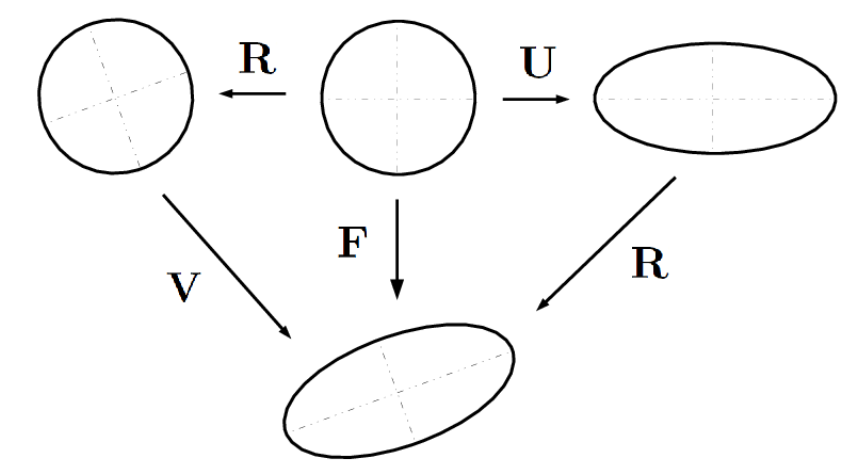
\includegraphics[width=0.7\textwidth]{figures/L2F1.png} 
     \caption{Under an invertible matrix $\mathbf{F}$ points a sphere is mapped to an ellipsoid. Using this
    fact, the geometric meaning of the polar decomposition theorem is shown. An
    undeformed circle is shown in the centre of the upper row, with the dashed lines
    along the eigenvectors of the symmetric matrix $\mathbf{U}$.}
     \label{fig:1}
 \end{figure}

\subsection*{Proof of the polar decomposition theorem - NON-EXAMINABLE}

You do not need to know the proof of this theorem, but it is simple enough to sketch for those interested. First we define a symmetric matrix
\begin{equation}
\mathbf{C} = \mathbf{F}^{T}\mathbf{F},
\end{equation}
which is positive-definite because $\mathbf{F}$ is invertible. It follows that the square root of $\mathbf{C}$ can be
 defined\footnote{This is done by first diagonalising $\mathbf{C} = \mathbf{Q} \text{diag}(\lambda_1, \lambda_2, \lambda_3) 
 \mathbf{Q}^T$ with $\mathbf{Q}$ orthogonal, and then setting $\mathbf{U} = \mathbf{Q} \text{diag}(\sqrt{\lambda_1}, \sqrt{\lambda_2}, 
 \sqrt{\lambda_3}) \mathbf{Q}^T$ which is well-defined as the eigenvalues are all positive.}, and we set $\mathbf{U} = \sqrt{\mathbf{C}}$ which
  is symmetric and positive-definite by construction. Our claim is that $\mathbf{R} = \mathbf{F}\mathbf{U}^{-1}$ is a rotation matrix. This 
  requires that $\mathbf{R}^{T}\mathbf{R} = \mathbf{I}$ and also $\det \mathbf{R} = 1$. For the first identity we have
\begin{equation}
\mathbf{R}^{T}\mathbf{R} = \mathbf{U}^{-1}\mathbf{F}^{T}\mathbf{F}\mathbf{U}^{-1}
\end{equation}
but $\mathbf{F}^{T}\mathbf{F} = \mathbf{C} = \mathbf{U}^2$, and hence $\mathbf{R}^{T}\mathbf{R} = \mathbf{I}$ as required. For
 the determinant condition we note that $\det(\mathbf{R}) = \frac{\det \mathbf{F}}{\det \mathbf{U}}$, while $\mathbf{U}^2 = 
 \mathbf{F}^T\mathbf{F}$ implies $\det \mathbf{U} = |\det \mathbf{F}|$. Since we assume $\det \mathbf{F} > 0$, we have $\det \mathbf{R} = 1$.
  For the second identity, we merely note that
\begin{equation}
\mathbf{F} = \mathbf{R}\mathbf{U} = \mathbf{R}\mathbf{U}\mathbf{R}^T\mathbf{R}
\end{equation}
and define $\mathbf{V} = \mathbf{R}\mathbf{U}\mathbf{R}^T$ which is just $\mathbf{U}$ rotated and so has the same eigenvalues.

\section*{Implications for the strain energy function}

Using the polar decomposition theorem, the deformation gradient can be written
\begin{equation}
\mathbf{F} = \mathbf{R}\mathbf{U}
\end{equation}
with $\mathbf{R}$ a rotation matrix, while $\mathbf{U} = \sqrt{\mathbf{C}}$ with $\mathbf{C} = \mathbf{F}^{T}\mathbf{F}$. It follows from eq.(1) that
\begin{equation}
W(\mathbf{x}, \mathbf{F}) = W(\mathbf{x}, \mathbf{R}\mathbf{U}) = W(\mathbf{x}, \mathbf{U}),
\end{equation}
and we conclude that the strain energy depends on the deformation gradient only through the symmetric matrix $\mathbf{U}$,
 or equivalently on $\mathbf{C}$. Within continuum mechanics, the symmetric matrix
\begin{equation}
\mathbf{C} = \mathbf{F}^{T}\mathbf{F}
\end{equation}
is known as the \textbf{right Cauchy-Green deformation tensor}\footnote{$\mathbf{F}\mathbf{F}^T$ is the
 \textbf{left Cauchy-Green deformation} tensor which is useful in some circumstances.}. To summarise, we have shown 
 that a strain energy function satisfies the principle of material frame indifference if and only if it takes the form
\begin{equation}
W(\mathbf{x}, \mathbf{F}) = \mathcal{U}(\mathbf{x}, \mathbf{C}),
\end{equation}
where $\mathcal{U}$ is some auxiliary strain energy function dependent on the right Cauchy-Green deformation tensor. Note that we use $\mathbf{C}$ instead of $\mathbf{U}$ in this formula because it simplifies later calculations.

Combining eq. (9) with the definition of the first Piola-Kirchhoff stress tensor
\begin{equation}
T_{ij} = \frac{\partial W}{\partial F_{ij}}
\end{equation}
we use the chain rule to obtain
\begin{equation}
T_{ij} = \frac{\partial \mathcal{U}}{\partial C_{kl}}\frac{\partial C_{kl}}{\partial F_{ij}}.
\end{equation}
From the definition of the right Cauchy-Green deformation tensor, a routine calculation shows that
\begin{equation}
\frac{\partial C_{kl}}{\partial F_{ij}} = \frac{\partial}{\partial F_{ij}}(F_{mk}F_{ml}) = \delta_{im}\delta_{jk}F_{ml} + F_{mk}\delta_{im}\delta_{jl} = \delta_{jk}F_{il} + \delta_{jl}F_{ik},
\end{equation}
and using the symmetry of $\mathbf{C}$ we arrive at the identity
\begin{equation}
T_{ij} = 2F_{ik}\frac{\partial \mathcal{U}}{\partial C_{kj}}
\end{equation}
If we define the \textbf{second Piola-Kirchhoff stress tensor} to be
\begin{equation}
S_{ij} = 2\frac{\partial \mathcal{U}}{\partial C_{ij}}
\end{equation}
the first Piola-Kirchhoff stress tensor can be decomposed in the form
\begin{equation}
T_{ij} = F_{ik}S_{kj}
\end{equation}
or in matrix form as $\mathbf{T} = \mathbf{F}\mathbf{S}$. It is clear that $\mathbf{S}$ is a symmetric matrix,
 and so we see that the principle of material frame indifference implies that the following combination
\begin{equation}
\mathbf{F}^{-1}\mathbf{T}
\end{equation}
of the deformation gradient and the first Piola-Kirchhoff stress tensor is symmetric. In the first 
problem set you will show that this condition is equivalent to the conservation of angular momentum. It follows, therefore, 
that angular momentum is automatically conserved during the motion of a simple hyperelastic body\footnote{For those
 that know about such things, this also follows from Noether's theorem.}. Within other forms of
 continuum mechanics, such as for viscous fluids, angular momentum conservation needs to be explicitly imposed within the governing equations.

\section*{The equilibrium equations}

Within the last lecture, we showed  that the equations of motion for a simple hyperelastic body can be written
\begin{equation}
\rho\frac{\partial v_{i}}{\partial t} - \frac{\partial T_{ij}}{\partial x_{j}} = 0,
\end{equation}
and are subject to the traction-free boundary conditions
\begin{equation}
T_{ij}\hat{n}_{j} = 0.
\end{equation}
An equilibrium configuration $\bphi^0$ is a time-independent solution of these equations, and therefore satisfies
\begin{equation}
-\frac{\partial T_{ij}^{0}}{\partial x_{j}} = 0
\end{equation}
along with the boundary condition
\begin{equation}
T_{ij}^{0}\hat{n}_{j} = 0.
\end{equation}
Here we have defined the equilibrium first Piola-Kirchhoff stress tensor
\begin{equation}
T_{ij}^{0} = \frac{\partial W}{\partial F_{ij}}[\mathbf{x}, \mathbf{F}^0(\mathbf{x})],
\end{equation}
with $\mathbf{F}^0$ the deformation gradient of $\bphi^0$. Let $\bphi^0$ be an equilibrium configuration of a body. 
As the choice of reference body $M$ is arbitrary, we are free to require that for all $\mathbf{x} \in M$ we have
\begin{equation}
\bphi^0(\mathbf{x}) = \mathbf{x}.
\end{equation}
It follows that $\mathbf{F}^0(\mathbf{x}) = \mathbf{I}$, and recalling eq. (15) we see that at equilibrium the first 
and second Piola-Kirchhoff stresses are equal, and hence both are symmetric. 

We assume for the first part of this course that $\mathbf{T}^0(\mathbf{x}) = \mathbf{0}$ for every $\mathbf{x} \in M$
 which is a non-unique solution of the equations of motion in eq. (19) and the associated boundary conditions in eq.(20). 
 Such an equilibrium configuration is said to be stress-free, and corresponds physically to the equilibrium state being one 
 of minimum elastic potential energy. Prior to an earthquake, the Earth is certainly not stress-free, and we will return to this 
 issue later. For many applications, however, it turns out that the neglect of equilibrium stress is an acceptable approximation.

\section*{Linearised equations of motion}

We can now rapidly obtain the equations of motion about a stress-free equilibrium configuration. Suppose that at $t = 0$ the 
body is displaced from equilibrium, with the initial motion taking the form
\begin{equation}
\varphi_{i}(\mathbf{x}, 0) = x_{i} + s U_{i}(\mathbf{x})
\end{equation}
for some given vector $\mathbf{U}$, while for some $\mathbf{V}$ the initial velocity is given by
\begin{equation}
v_{i}(\mathbf{x}, 0) = s V_{i}(\mathbf{x}).
\end{equation}
Here $s$ is a dimensionless number that indicates the order of terms in a perturbation series. We shall assume that the 
subsequent motion can be expanded in powers of $s$, and hence seek a solution of the form
\begin{equation}
\varphi_{i}(\mathbf{x}, t) = x_{i} + s u_{i}(\mathbf{x}, t) + O(s^2)
\end{equation}
where $\mathbf{u}$ will be known as the \textbf{displacement vector} of the linearised motion. Working always to first-order 
in $s$, we find that the referential velocity of the motion is given by
\begin{equation}
v_{i} = s\frac{\partial u_{i}}{\partial t} + O(s^2)
\end{equation}
while the deformation gradient can be written
\begin{equation}
F_{ij} = \delta_{ij} + s\frac{\partial u_{i}}{\partial x_{j}} + O(s^2).
\end{equation}
Similarly, the first Piola-Kirchhoff stress tensor can be expanded as
\begin{equation}
T_{ij}(\mathbf{x}, t) = s\frac{\partial^2 W}{\partial F_{ij}\partial F_{kl}}(\mathbf{x}, \mathbf{I})\frac{\partial u_{k}}{\partial x_{l}} + O(s^2),
\end{equation}
where we have made use of our assumption that the equilibrium stress vanishes. It will be useful to define the elastic tensor by
\begin{equation}
A_{ijkl}(\mathbf{x}) = \frac{\partial^2 W}{\partial F_{ij}\partial F_{kl}}(\mathbf{x}, \mathbf{I}),
\end{equation}
so that we can write the stress tensor more concisely as
\begin{equation}
T_{ij} = s A_{ijkl}\frac{\partial u_{k}}{\partial x_{l}} + O(s^2).
\end{equation}
This linearised relationship is \textbf{Hooke's law}. But please note that this is not a "law" of nature nor an 
empirical result. It arises solely as an approximation to finite elasticity which is valid for sufficiently small 
displacements about equilibrium. Due to the equality of mixed partial derivatives, the elastic tensor $A_{ijkl}$ 
possesses the so-called \textbf{hyperelastic symmetry}
\begin{equation}
A_{ijkl} = A_{klij}.
\end{equation}
We shall see through this course that this innocuous looking symmetry plays a central role within the theory of elastic wave propagation!
 In the first problem set you will show that this tensor has additional symmetries
\begin{equation}
A_{ijkl} = A_{jikl} = A_{ijlk}
\end{equation}
that reduce the number of independent components from 45 to 21. In particular, the symmetry of the elastic tensor in its
final two indices means that
\begin{equation}
A_{ijkl}\frac{\partial u_{k}}{\partial x_{l}} = A_{ijkl}\frac{1}{2}\left(\frac{\partial u_{k}}{\partial x_{l}} + 
\frac{\partial u_{l}}{\partial x_{k}}\right)
\end{equation}
where on the right hand side we identify what is commonly called the strain tensor. More properly, this quantity is the 
\textbf{linearised strain tensor}, which is obtained through linearisation of the \textbf{finite-strain} $\mathbf{E} = \frac{1}{2}[\mathbf{C} - 
\mathbf{I}]$ which vanishes in the equilibrium configuration. It is possible to develop the general theory 
in terms of $\mathbf{E}$ and not $\mathbf{C}$ but there is little gained by doing this.


The exact equations of motion for the body are
\begin{equation}
\rho\frac{\partial v_{i}}{\partial t} - \frac{\partial T_{ij}}{\partial x_{j}} = 0.
\end{equation}
and are subject to the traction-free boundary conditions
\begin{equation}
T_{ij}\hat{n}_{j} = 0.
\end{equation}
Using the preceding expansions for $\mathbf{v}$ and $\mathbf{T}$ and equating first-order terms, we obtain the linearised equations of motion
\begin{equation}
\rho\frac{\partial^2 u_{i}}{\partial t^2} - \frac{\partial}{\partial x_{j}}\left(A_{ijkl}\frac{\partial u_{k}}{\partial x_{l}}\right) = 0
\end{equation}
along with the linearised boundary conditions
\begin{equation}
n_{j}A_{ijkl}\frac{\partial u_{k}}{\partial x_{l}} = 0.
\end{equation}
Eq.(36) and (37) are the basic equations governing elastic wave propagation, and in later lectures we will look at their properties. Within these equations there are two physical parameters; the density $\rho$, and the elastic tensor $\mathbf{A}$. Both are functions that can vary smoothly within the body. There might also be discontinuities in these parameters across internal surfaces such as the core-mantle boundary, across which continuity of displacement and traction must be imposed.

\section*{Material symmetries}

In general the elastic tensor has 21 independent components. In certain materials, however, this number is reduced due to 
the presence of \textbf{material symmetries}. Let us fix a point $\mathbf{x}$, and suppose there is a rotation matrix $\mathbf{Q}$ such that
\begin{equation}
W(\mathbf{x}, \mathbf{F}\mathbf{Q}) = W(\mathbf{x}, \mathbf{F}),
\end{equation}
for any deformation gradient $\mathbf{F}$. Using the second part of the polar decomposition theorem we
 have $\mathbf{F} = \mathbf{V}\mathbf{R}$, with $\mathbf{V}$ symmetric and positive-definite, while $\mathbf{R}$ is a
  rotation matrix. It follows that $\mathbf{F}$ and $\mathbf{F}\mathbf{Q}$ represent the same magnitude of stretching,
   but oriented about different axes. Thus we can say that in eq. (38) there is a symmetry of the strain energy with 
   respect to \emph{orientation of stretching}. The collection of all such rotation matrices forms the \textbf{material symmetry 
   group}\footnote{If you care to, check that this really is a group.} at the point $\mathbf{x}$. 
   
   If the material symmetry 
   group at $\mathbf{x}$ comprises all rotation matrices, we say that the material is \textbf{isotropic} at this point. If the material 
   is not isotropic, then it is \textbf{anisotropic}. The crystalline materials that make up the Earth's interior are almost always 
   quite strongly anisotropic. However, seismic waves have wavelengths substantially larger than individual crystals, and so they ``see'' an 
   average over many crystals with many different orientations. The end result is that for most seismological applications the Earth 
   appears to be either isotropic or only slightly anisotropic.

\subsection*{Isotropic materials}

Given their practical relevance, let us consider isotropic materials in further detail. To simplify notations, 
we work at a fixed point $\mathbf{x}$, and suppress this dependence within the formulae. By assumption the strain energy of an 
isotropic material satisfies
\begin{equation}
W(\mathbf{F}\mathbf{Q}) = W(\mathbf{F}),
\end{equation}
for all $\mathbf{F}$ and any rotation matrix $\mathbf{Q}$. From material frame indifference, however, we know that we can always write
\begin{equation}
W(\mathbf{F}) = \mathcal{U}(\mathbf{C})
\end{equation}
with $\mathbf{C} = \mathbf{F}^{T}\mathbf{F}$. And hence for an isotropic material we must have
\begin{equation}
\mathcal{U}(\mathbf{C}) = \mathcal{U}(\mathbf{Q}^{T}\mathbf{C}\mathbf{Q}).
\end{equation}
Because $\mathbf{C}$ is symmetric, the matrix $\mathbf{Q}^{T}\mathbf{C}\mathbf{Q}$ can be made diagonal for
 an appropriate choice of rotation matrix $\mathbf{Q}$. We conclude that in an isotropic material the strain 
 energy depends \emph{only on $\mathbf{C}$ through its eigenvalues}. Using this result it is only a matter of tedious algebra (which we will skip) to obtain the general form of the elastic tensor in an isotropic material. The end result is that
\begin{equation}
A_{ijkl} = \lambda\delta_{ij}\delta_{kl} + \mu(\delta_{ik}\delta_{jl} + \delta_{il}\delta_{kj}),
\end{equation}
where $\lambda$ and $\mu$ are collectively known as the \textbf{Lamé parameters}, and $\mu$ is 
called the \textbf{shear modulus}. If it is also assumed that the Lamé parameters are constant, it can readily be shown that
 the linearised equations of motion reduce to
\begin{equation}
\rho\frac{\partial^2 \mathbf{u}}{\partial t^2} - (\lambda + \mu)\nabla(\nabla\cdot \mathbf{u}) - \mu\nabla^2 \mathbf{u} = 0.
\end{equation}
This is the form of the equations of elasticity covered in the 1B dynamics course. 

For reference, note that the isotropic elastic tensor can also be expressed using the shear modulus along with the \textbf{bulk modulus}
 $K$ which is defined in terms of $\lambda$ and $\mu$ through
\begin{equation}
\kappa = \lambda + \frac{2}{3}\mu.
\end{equation}
As a comment, you might ask why I have taken almost two lectures to get to an equation most of you will already know! There are 
two reasons. First, eq.(43) is not the equation of motion for a general elastic body, but for the linearised motion subject to a 
whole host of simplifying assumptions (e.g. isotropy, homogeneity, no initial stress, no gravitation). Such assumptions are generally 
invalid within seismological applications, and hence we do practically need to consider more general formulations. But beyond this, I 
think it is always better to have stated clearly and precisely what has and has not been assumed within a physical theory.

\subsection*{Transversely isotropic materials}

We describe briefly an important class of anisotropic materials. Let $\hat{\boldsymbol{\nu}}$ be a unit vector, 
and suppose that eq.(39) holds for all rotation matrices $\mathbf{Q}$ that leave $\hat{\boldsymbol{\nu}}$ fixed. Such a 
strain energy function is said to be \textbf{transversely isotropic} with symmetry axis $\hat{\boldsymbol{\nu}}$. The most general 
strain energy function consistent with this condition has been determined, and it can be shown that the resulting elastic tensor 
takes the following form
\begin{equation}
\begin{split}
A_{ijkl} = &\lambda\delta_{ij}\delta_{kl} + \mu(\delta_{ik}\delta_{jl} + \delta_{il}\delta_{kj}) + 8\gamma\hat{\nu}_{i}\hat{\nu}_{j}\hat{\nu}_{k}\hat{\nu}_{l} + 4\xi(\hat{\nu}_{i}\hat{\nu}_{j}\delta_{kl} + \delta_{ij}\hat{\nu}_{k}\hat{\nu}_{l}) \\
&-\zeta(\hat{\nu}_{i}\hat{\nu}_{k}\delta_{jl} + \hat{\nu}_{j}\hat{\nu}_{k}\delta_{il} + \hat{\nu}_{j}\hat{\nu}_{l}\delta_{ik} + \hat{\nu}_{i}\hat{\nu}_{l}\delta_{jk}),
\end{split}
\end{equation}
where $\lambda$ and $\mu$ are as before, while $\gamma, \xi$, and $\zeta$ are additional elastic modulii. Do not fear, 
you do not need to remember any such complicated tensor expressions! The point here is just to indicate concretely that 
there is more to the world than isotropic elasticity.

\subsection*{Elastic fluids}

The discussion of material symmetries above actually applies only to solids. There is, however, an 
extension of these ideas to so-called \textbf{elastic fluids}. This means that the fluid is assumed to be compressible, 
but to have no viscosity. Within seismological applications this is a good approximation when considering wave propagation within 
the oceans or in the Earth's outer core. All our basic equations already apply to elastic fluids, and the only difference 
is the form of the strain energy function. We stated in the previous lecture that an elastic body has a preferred shape 
and/or volume. In an elastic fluid, however, there is only a preferred volume. This means that \emph{deformations that leave the 
volume fixed have no effect on the strain energy}. Mathematically this is expressed by requiring that
\begin{equation}
W(\mathbf{x}, \mathbf{F}\mathbf{Q}) = W(\mathbf{x}, \mathbf{F}),
\end{equation}
for all $\mathbf{F}$ and all matrices $\mathbf{Q}$ with determinant equal to one\footnote{If you know some group theory, we can say that an elastic fluid has symmetry group equal to SL(3), while for a solid the symmetry group is a subgroup of SO(3). It can be shown that there is no proper subgroup intermediate between SO(3) and SL(3), and hence there is no "intermediate" state between solids and fluids. This approach to classifying elastic materials is due to Walter Noll (1925-2017).}. It follows readily that the strain energy depends on $\mathbf{F}$ only through its determinant, and hence we can write
\begin{equation}
W(\mathbf{x}, \mathbf{F}) = \mathcal{V}(\mathbf{x}, J),
\end{equation}
for some function $\mathcal{V}$, where $J = \det(\mathbf{F})$. In terms of the linearised theory, it is then a matter of algebra to show that the elastic tensor takes the form
\begin{equation}
A_{ijkl} = \kappa\delta_{ij}\delta_{kl}
\end{equation}
which is that of an isotropic solid but with vanishing shear modulus.

\section*{What you need to know and be able to do}

\begin{itemize}
    \item[(i)] The statement of the polar decomposition theorem, and how this can be used to restrict the allowable form of the strain energy function. The proof of the polar decomposition theorem is non-examinable.
    \item[(ii)] What a stress-free equilibrium configuration is, and how to derive the linearised equations of motion for small disturbances about such a configuration. Within this course, you will become very familiar with these linearised equations of motion, and it will be necessary to memorise their form (in the non-gravitating case discussed in this lecture) for the exam.
    \item[(iii)] The definition of the material symmetry group, and its physical interpretation.
    \item[(iv)] The meaning of the terms elastic solid, elastic fluid, isotropic, anisotropic, and transversely isotropic. You do not need to remember the form of the elastic tensor in any particular case, but you should memorise the hyperelastic symmetry $A_{ijkl} = A_{klij}$ due to its great physical importance.
\end{itemize}

\end{document}
